% Part B: accepted computational design and explicitly predicted experiments.
\subsection{Computed Construct and Experimental Predictions}
The in-silico \ConstructName{} (\ConstructBp{} bp; Figure~\ref{fig:plasmid}) encodes a \FusionAa{}-residue TFEB--EGFP fusion: \TFEBAa{} TFEB residues, the seven-residue \LinkerPeptide{} junction, and \EGFPAa{} EGFP residues. The native TFEB stop is absent; EGFP supplies the final TAA. The calculated unmodified average mass is \FusionMassKDa{} kDa.

The reconstruction and an independent standard-library audit agreed on sequence, reading frame, junctions, terminal stop and fragment geometry. Corresponding checks rejected four software challenges: reversed TFEB, a one-base frameshift, restored native TFEB stop, and an internal HindIII site. These are not experimental clones or a measured success rate.

\begin{figure}[htbp]
\centering
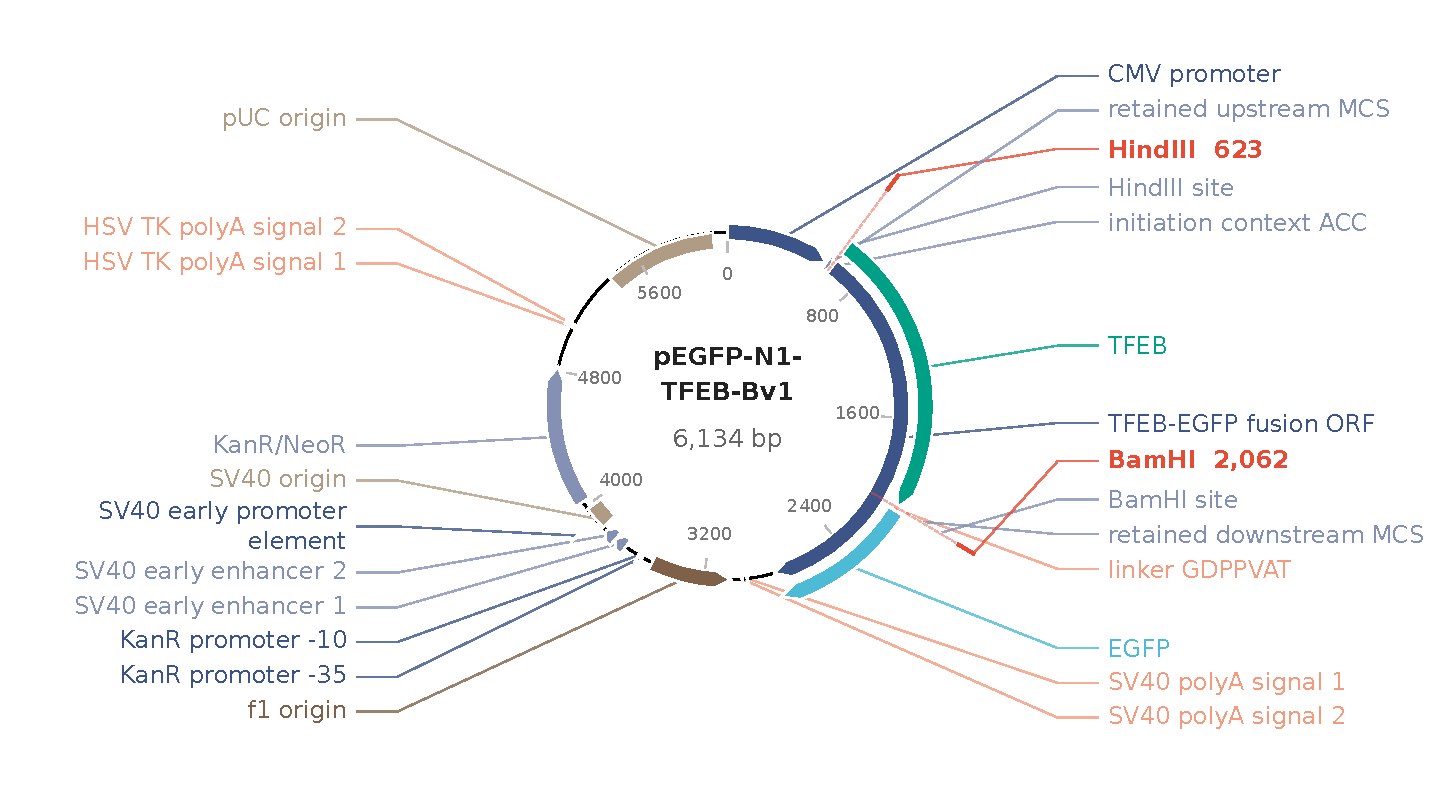
\includegraphics[width=\textwidth]{images/B/plasmid-map.pdf}
\caption{Predicted annotation map of \ConstructName{} (\ConstructBp{} bp), rendered from the accepted GenBank sequence. The complete fusion ORF overlaps its TFEB, linker and EGFP components intentionally. HindIII 623 and BamHI 2062 denote the first reference-strand nucleotide after cleavage; their recognition sequences begin at 622 and 2061, respectively. Poly(A) annotations are signal motifs, not complete processing regions. KanR applies to bacteria and Neo/G418 to mammalian selection. The pUC and SV40 origins are shown without an inferred directional arrow. No experimental observation is represented.}
\label{fig:plasmid}
\end{figure}

Cloning PCR predicts a \PCRBp{} bp product. HindIII/BamHI digestion yields a \InsertBp{} nt insert and \BackboneBp{} nt backbone by the cut-to-cut single-strand convention. Their pydna duplex spans are 1,443 and 4,699 bp, including four-base overhangs; gel sizes use the nominal single-strand lengths. Because the empty vector loses a \RemovedMCSBp{} nt MCS segment, the final length is not the intact vector length plus the undigested amplicon.

% Values transcribed from the P6-accepted expected_fragments.tsv.
Table~\ref{tab:screening} and Figure~\ref{fig:bands} summarize screening. Flanking PCR distinguishes insert-bearing candidates from empty vector. A negative orientation assay is read together with an amplification-positive control. If all orientation assays are negative in the first round, flanking-positive candidates go to sequencing. Reverse TFEB is a hypothetical challenge; incompatible-end directional ligation does not favor it.

\begin{table}[htbp]
\centering\small
\caption{Predicted screening products. All sizes are nominal bp; ``none'' means no specific product is predicted. R and S are hypothetical challenge sequences.}
\label{tab:screening}
\begin{tabularx}{\textwidth}{@{}L{3.2cm}YYY@{}}
\toprule
Sample & Flanking PCR (S-F1/S-R1) & Orientation PCR (S-F2/S-R1) & HindIII/BamHI digest \\
\midrule
Intended construct (C) & 2,605 & 2,093 & 4,695 + 1,439 \\
Empty vector (E) & 1,204 & none & 4,695 + 38 \\
Reverse TFEB (R) & 2,605 & none & 4,695 + 1,439 \\
Retained TFEB stop (S) & 2,608 & 2,096 & 4,695 + 1,442 \\
\bottomrule
\end{tabularx}
\end{table}

Flanking PCR and HindIII/BamHI digestion do not separate reversed TFEB from the intended construct, and the three-base retained-stop difference falls below gel resolution. Acceptance therefore rests on the expected digest plus actual, unambiguous, concordant bidirectional sequence across 602--2799 (2,198 nt), including both junctions, the complete fusion ORF and terminal stop. Ten primers predict usable coverage in both directions at every target base. Low-quality calls, mixed peaks, gaps and unexpected target changes are resolved under the Sanger acceptance procedure before cell assays. Figure~\ref{fig:workflow} summarizes the planned workflow and controls.


\begin{figure}[htbp]
\centering
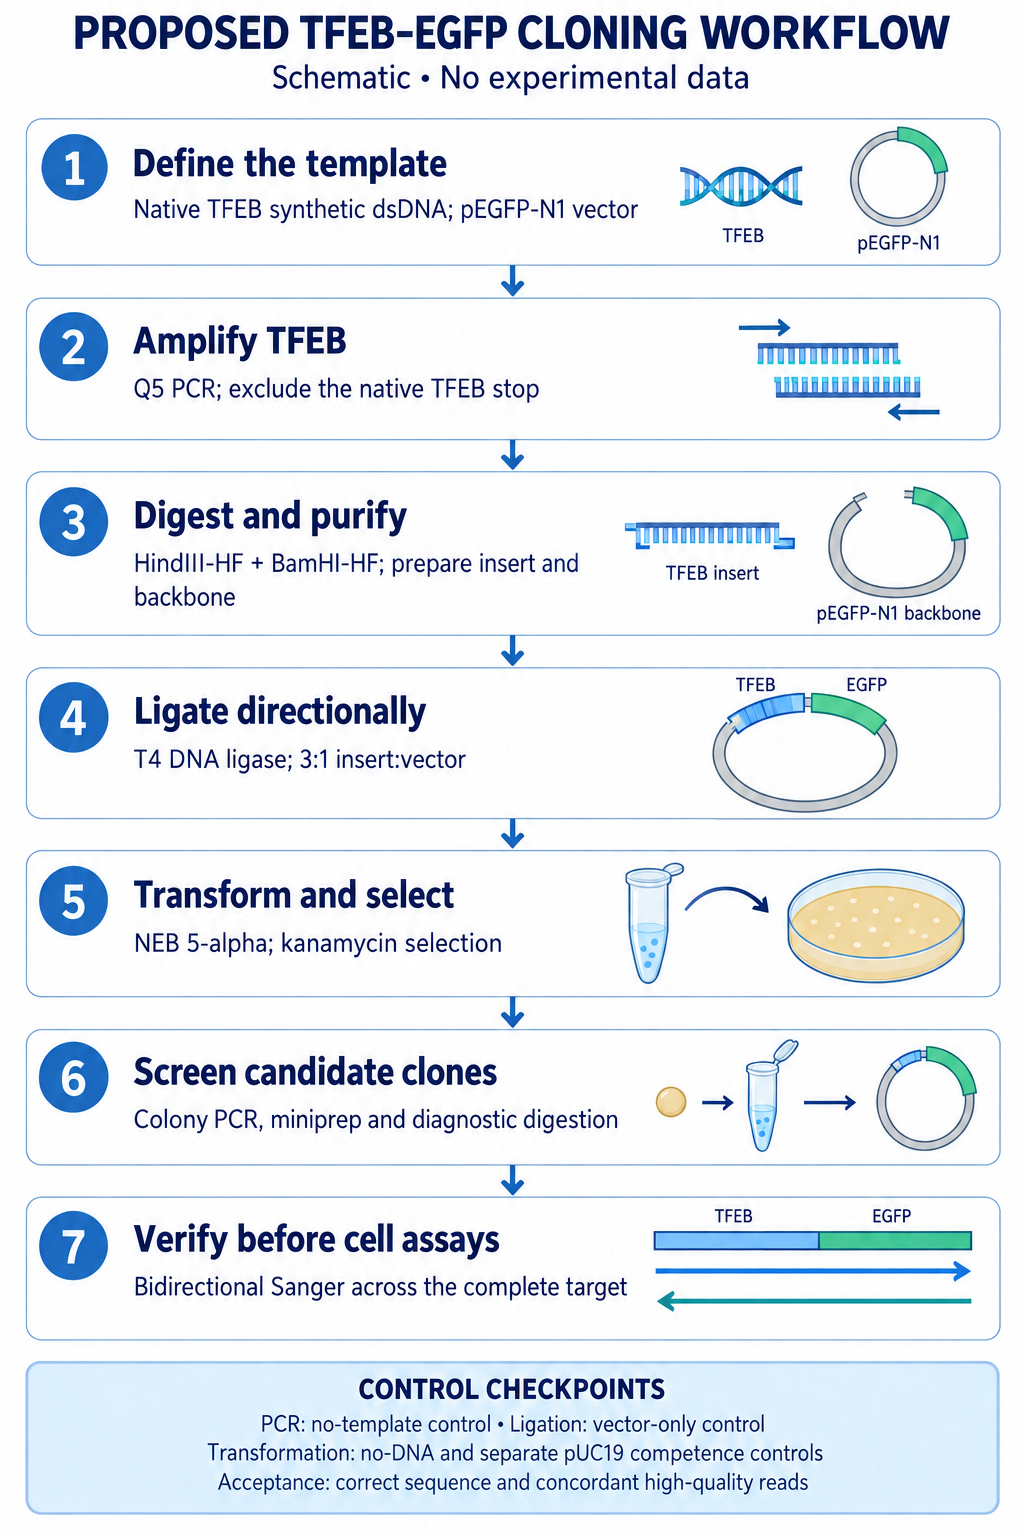
\includegraphics[width=0.92\textwidth,height=0.77\textheight,keepaspectratio]{images/B/cloning-workflow-imagegen-v2.png}
\caption{Proposed cloning workflow and control checkpoints. AI-assisted illustrations are symbolic, not exact molecular geometry, plasmid coordinates or experimental data. The full-length paired arrows summarize the intended bidirectional sequencing coverage, not observed reads. Each operation is planned; measured DNA concentrations and actual sequence quality are required before clone acceptance.}
\label{fig:workflow}
\end{figure}

\begin{figure}[htbp]
\centering
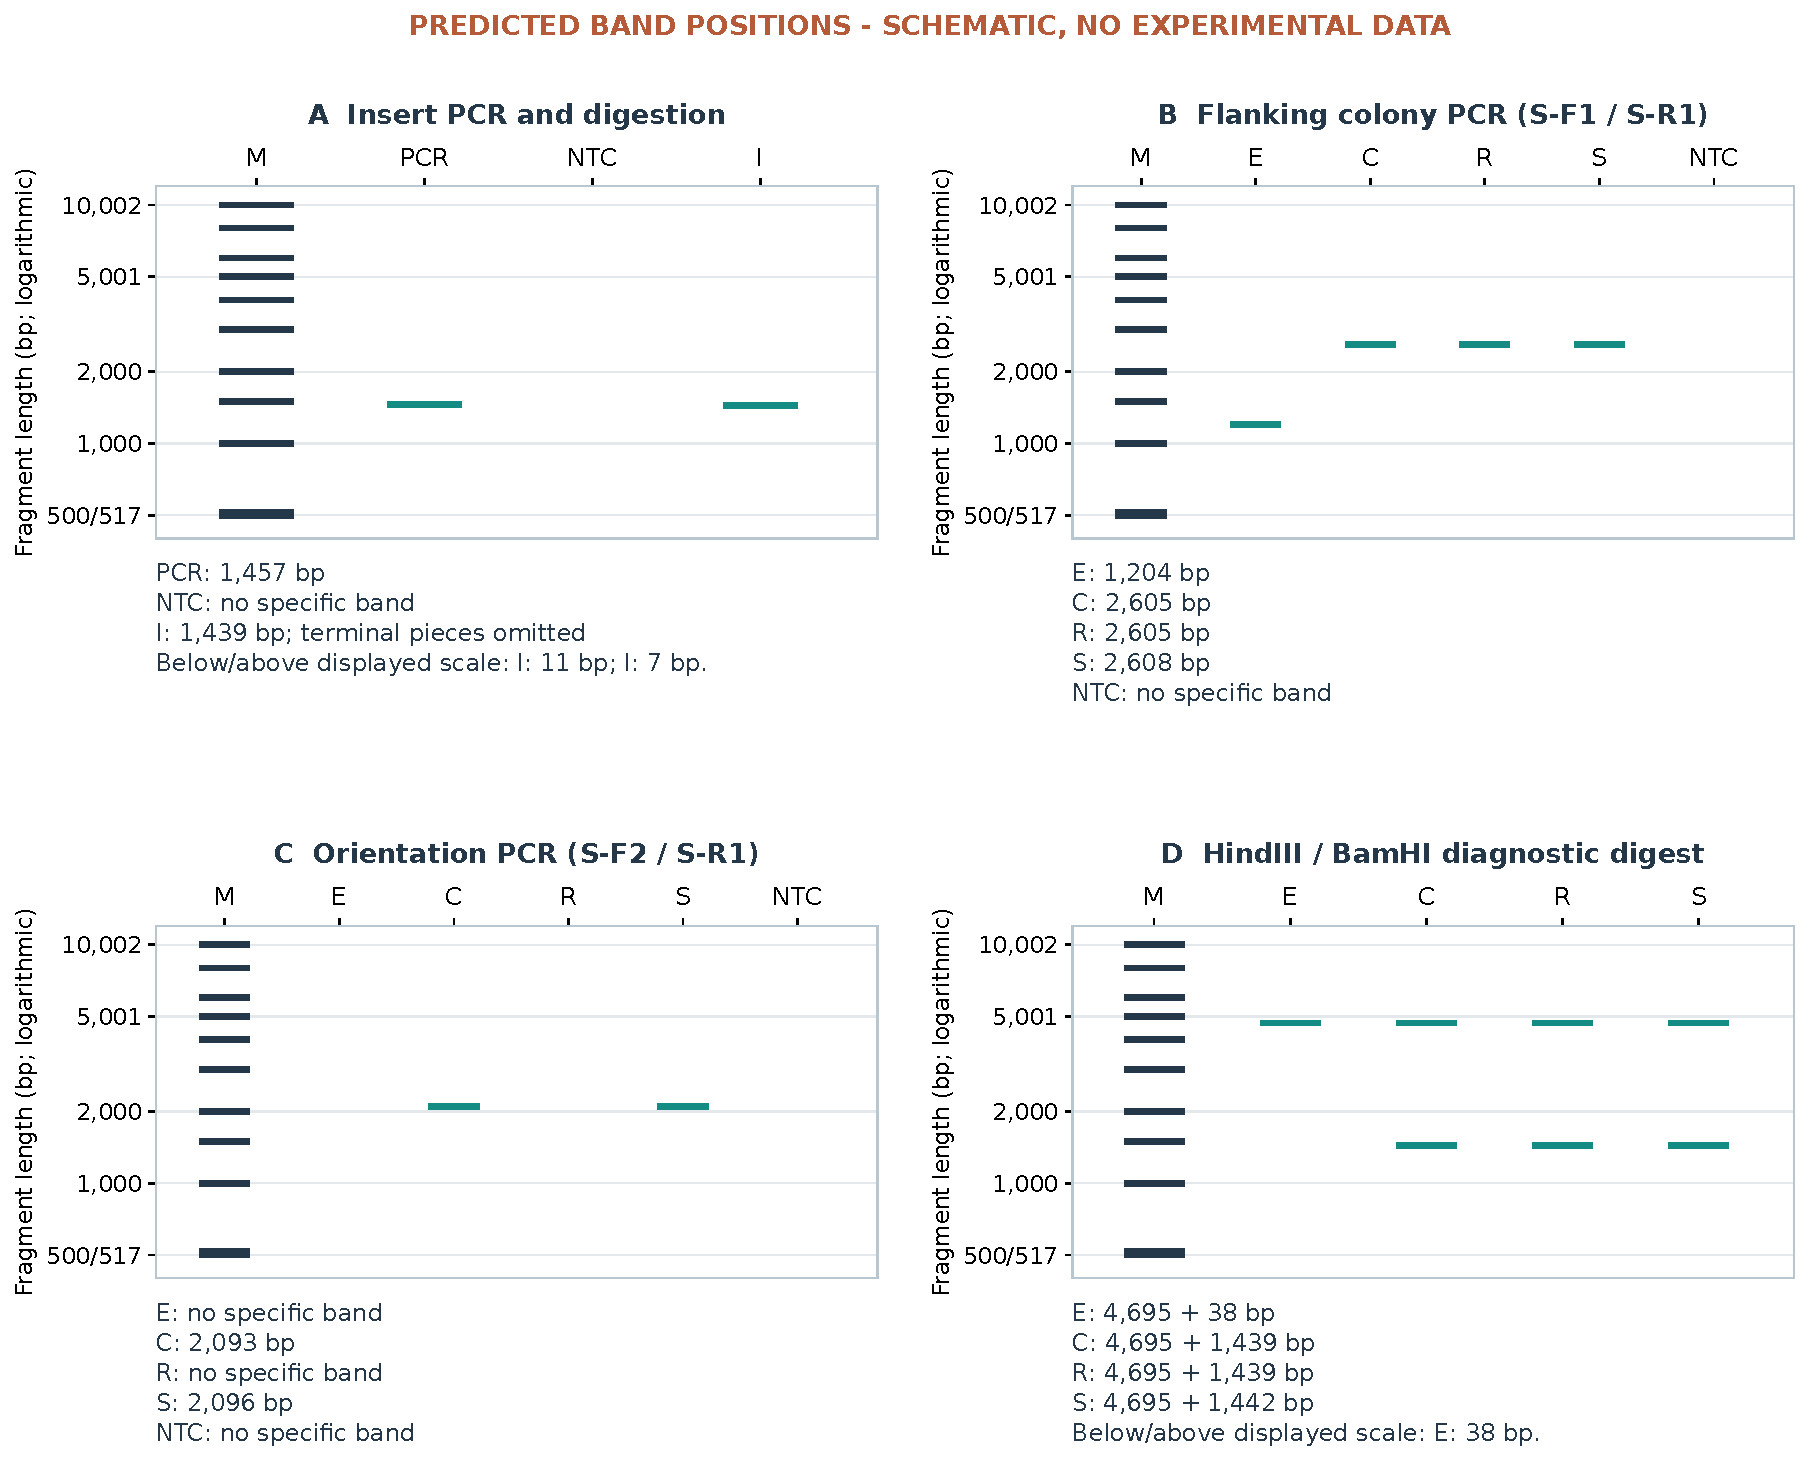
\includegraphics[width=\textwidth]{images/B/predicted-bands.pdf}
\caption{Predicted DNA-band positions, drawn as a schematic rather than an experimental gel. M: NEB N3232 ladder; PCR: tailed insert amplicon; I: digested insert; NTC: no-template control; E: empty vector; C: intended construct; R: hypothetical reverse-TFEB model; S: hypothetical retained-stop model. The 500/517 bp marker pair is not resolved~\cite{MethodM16}. The 7, 11 and 38 nt fragments fall below the displayed range. Three-base differences between C and S are not expected to resolve on the proposed 1\% gel. An empty NTC schematic means no specific product is predicted, not a guarantee of a clean experimental lane. Uncut circular DNA mobility and band intensity are not predicted.}
\label{fig:bands}
\end{figure}
\FloatBarrier
